%%%%%%%%%%%%%%%%%%%%%%%%%%%%%%%%%%%%%%%%%%%%%%%%%%%%%%%%%%%%%%%%%%%%%%%%%%%%%%%%%%%%%%%%%
%%%  PREÂMBULO  %%%
%%%%%%%%%%%%%%%%%%%%%%%%%%%%%%%%%%%%%%%%%%%%%%%%%%%%%%%%%%%%%%%%%%%%%%%%%%%%%%%%%%%%%%%%%

\documentclass[12pt,openright,twoside,a4paper,sumario=tradicional,english,brazil]{abntex2}

%%% -----
%%% PACOTES
%%% -----

% Pacotes gerais
\usepackage[T1]{fontenc}
\usepackage[utf8]{inputenc}
\usepackage[pdftex]{graphicx}    % inserir figuras
\usepackage[alf,abnt-missing-year=sd]{abntex2cite}    % citação conforme as normas ABNT

\usepackage{indentfirst}         % indentação do primeiro parágrafo
\usepackage{pdfpages}            % inserir páginas em pdf (e.g. ficha catalográfica)
\usepackage{setspace}            % para definir espaçamento entre linhas

\usepackage{microtype}           % quebrar citações para não ultrapassar margem da página
\usepackage{xurl}                % quebrar url para não ultrapassar margem da página

\usepackage{lastpage}            % capturar a última página
\usepackage{placeins}            % controlar posição das tabelas

% Pacotes para construção de tabelas
\usepackage{booktabs}
\usepackage{longtable}
\usepackage{array}
\usepackage{multirow}
\usepackage{tabularx}
\usepackage{float}
\usepackage{colortbl}
\usepackage{pdflscape}
\usepackage{threeparttable}
\usepackage{threeparttablex}
\usepackage{makecell}
\usepackage{xcolor}

% Aumentar espaçamento entre capítulos no sumário

% Declarar caracteres especiais
\DeclareUnicodeCharacter{2500}{\mbox{\vrule height2.2ptdepth-1.8ptwidth.5em}} % declarar travessão

%%% -----
%%% CONFIGURAÇÕES
%%% -----

\graphicspath{{./figuras/}}   

%%% -----
%%% CUSTOMIZAÇÕES
%%% -----

% Modificar fonte da tese
\usepackage{courier}  % usa o Adobe Courier no lugar de Computer Modern
\fontfamily{courier}\selectfont

% Modificar fonte e tamanho dos capítulos
\renewcommand{\ABNTEXchapterfontsize}{\huge}
\renewcommand{\ABNTEXchapterfont}{\fontfamily{lmr}\fontseries{sb}\selectfont}

% Separar numeração de figuras e tabelas por capítulo
\counterwithin{figure}{chapter}
\counterwithin{table}{chapter}

\floatstyle{plaintop} % mudar a posição das legendas das tabelas para cima
\restylefloat{table}  % mudar a posição das legendas das tabelas para cima

\hypersetup{hidelinks}   % to remove ugly boxes from hyperlinks (cross-references)

% Configurar legendas
\usepackage[font=small,format=plain,labelfont=bf,up,textfont=up]{caption}

\raggedbottom                                   % não permitir espaços extra no texto
\setlength{\cftbeforechapterskip}{\onelineskip} % aumentar espaçamento entre capitulos no sumário

% Criar um estilo para os capítulos
\makeatletter
\newcommand\thickhrulefill{\leavevmode \leaders \hrule height 1ex \hfill \kern \z@}
\setlength\midchapskip{10pt}
\makechapterstyle{custom}{
\renewcommand\chapternamenum{}
\renewcommand\printchaptername{}
\renewcommand\chapnamefont{\Large\scshape}
\renewcommand\printchapternum{%
\chapnamefont\null\thickhrulefill\quad
\@chapapp\space\thechapter\quad\thickhrulefill}
\renewcommand\printchapternonum{%
\par\thickhrulefill\par\vskip\midchapskip
\hrule\vskip\midchapskip
}
\renewcommand\chaptitlefont{\Large\scshape\centering}
\renewcommand\afterchapternum{%
\par\nobreak\vskip\midchapskip\hrule\vskip\midchapskip}
\renewcommand\afterchaptertitle{%
\par\vskip\midchapskip\hrule\nobreak\vskip\afterchapskip}
}
\makeatother

%%% -----
%%% Formato de cabeçalho/rodapé romano nos elementos pré-textuais
%%% -----

%% Novo estilo
\makepagestyle{estilo_pretextual} %%% escolha um nome
  \makeevenhead{estilo_pretextual}{}{}{\ABNTEXfontereduzida \textbf \thepage}
  \makeoddhead{estilo_pretextual}{}{}{\ABNTEXfontereduzida \textbf \thepage}

% ---
% Inserir algarismos romanos nos elementos pré-textuais
\renewcommand{\pretextual}{
  \pagenumbering{roman} %%% ou \pagenumbering{Roman}
  \aliaspagestyle{chapter}{estilo_pretextual}% customizing chapter pagestyle
  \pagestyle{estilo_pretextual}
  \aliaspagestyle{cleared}{empty}
  \aliaspagestyle{part}{estilo_pretextual}
}

% Ajusta a marca \textual para que a numeração volte a ser arábica nos elementos textuais
\let\oldtextual\textual
\renewcommand{\textual}{%
  \oldtextual%
  \renewcommand{\thepage}{\arabic{page}}
}
% ---

% --------------------------------------------------------------------------------------
% VARIÁVEIS
% --------------------------------------------------------------------------------------

\instituicao{%
Universidade de São Paulo
\par
Instituto de Biociências
\par
Programa de Pós-Graduação em Genética e Biologia Evolutiva}

\titulo{Influência da seleção natural em populações nativas de diferentes ecorregiões americanas}
\tituloestrangeiro{Influence of natural selection on native populations from distinct American ecoregions}

\autor{Cainã Max Couto da Silva}
\orientador{Tábita Hünemeier}

\local{São Paulo}
\data{2021}

\tipotrabalho{Tese (Doutorado)}

\preambulo{Tese apresentada ao Instituto de Biociências da Universidade de São Paulo, para a obtenção de Título de Doutor em Ciências, na Área de Genética e Biologia Evolutiva.}

%%%%%%%%%%%%%%%%%%%%%%%%%%%%%%%%%%%%%%%%%%%%%%%%%%%%%%%%%%%%%%%%%%%%%%%%%%%%%%%%%%%%%%%%%
%%%  BEGIN DOCUMENT  %%%
%%%%%%%%%%%%%%%%%%%%%%%%%%%%%%%%%%%%%%%%%%%%%%%%%%%%%%%%%%%%%%%%%%%%%%%%%%%%%%%%%%%%%%%%%

\begin{document} 

\imprimircapa
\imprimirfolhaderosto*

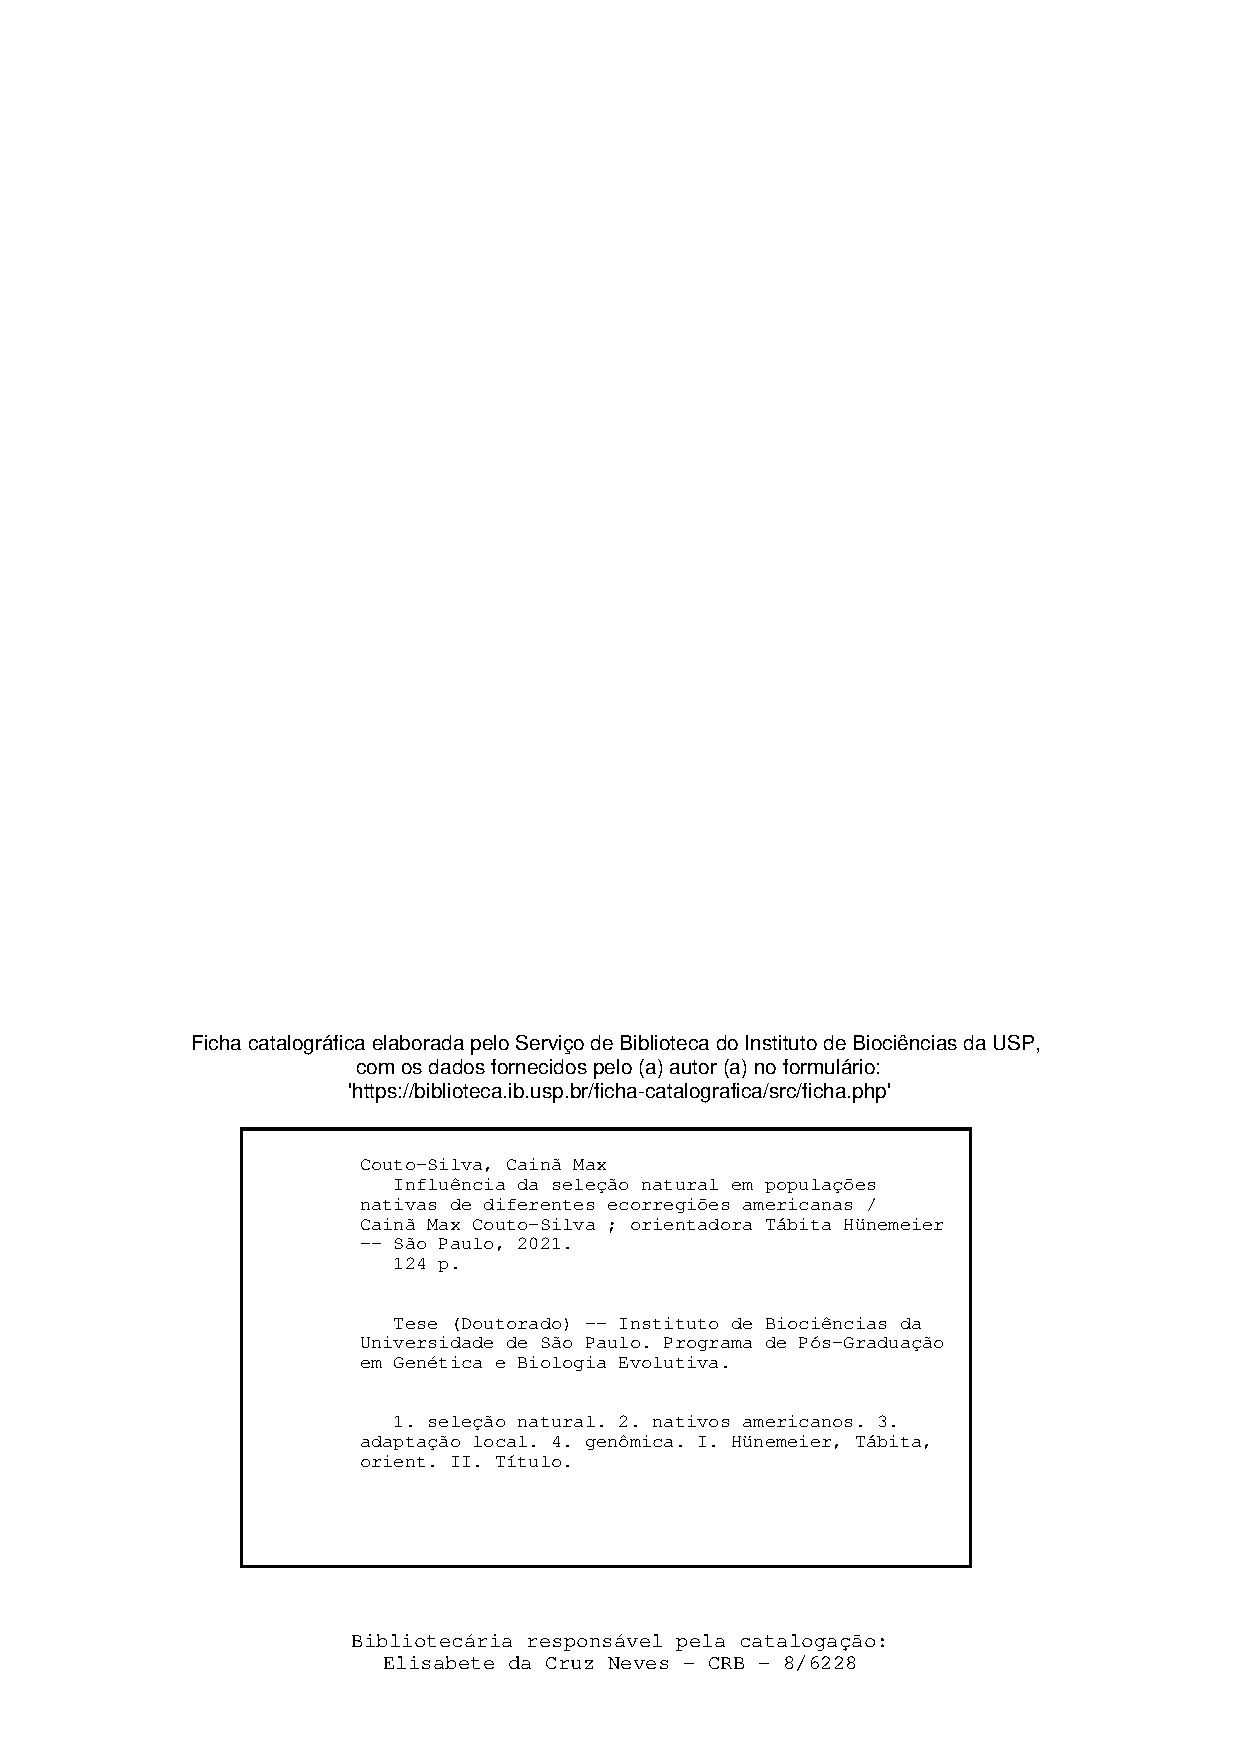
\includepdf{ficha_catalografica.pdf}

% --------------------------------------------------------------------------------------
% DEDICATÓRIA
% --------------------------------------------------------------------------------------

\begin{dedicatoria}
\vspace*{\fill}
\begin{flushright}
Dedico este trabalho ao meu filho de quatro patas, meu melhor amigo e fiel companheiro, que encheu meu coração de amor e ternura, Darwin.
\vspace{2cm}
\end{flushright}
\end{dedicatoria}

% --------------------------------------------------------------------------------------
% AGRADECIMENTOS
% --------------------------------------------------------------------------------------

\begin{agradecimentos}

\setlength{\parindent}{1.5cm}  % Parágrafo com 2cm de identação
\setlength{\parskip}{5pt}      % Espaçamento entre parágrafos

À minha orientadora, Tábita Hünemeier, pela orientação, pelas discussões científicas, pela compreensão, e por todas as oportunidades incríveis de aprendizagem dentro e fora do país.

Ao Prof. Dr. David Comas, por me receber de braços abertos para estágio em seu laboratório em Barcelona. E ao pós-doutorando André Flores, que esteve comigo no laboratório de Comas e contribuiu grandemente para o meu desenvolvimento acadêmico.

À todos os pesquisadores de campo que coletaram os dados, principalmente o Prof. Dr. Francisco Maurício Salzano (\emph{in memoriam}), que coletou a maioria das amostras analisadas neste trabalho, e teve um papel fundamental na genética de populações no Brasil.

À toda equipe envolvida no Departamento de Genética e Biologia Evolutiva do Instituto de Biociências da Universidade de São Paulo, pela infraestrutura e serviços prestados.

À CAPES e FAPESP (processo 2017/14916-8) pelas bolsas concedidas e auxílio financeiro para execução desta pesquisa.

À todos os meus colegas de laboratório, Renan Lemes, Marcos Silva, Tiago Silva, Maíra Rodrigues e Gabrielle Rizzato, pelas discussões científicas e todos os bons momentos ao longo do percurso do meu doutorado. Destaco a contribuição especial de Renan Lemes tanto para meu desenvolvimento acadêmico-profissional, como para a elaboração desta tese.

À toda equipe de docentes e discentes do “porão”, local principal onde foi desenvolvida minha pesquisa. Em especial ao André Fonseca, pelas discussões e bons momentos de confraternização.

Aos meus amigos que sempre me apoiaram e fazem parte da minha família, Rafael Santos, Rafael Pinheiro, Diego Silva, Leonardo Jackson, Caio Mendonça, Júlio Afonso e César Henrique.

À minha irmã de consideração, Magna Magalhães, por estar presente em minha vida desde o mestrado, e ter me auxiliado nos momentos mais difíceis.

À Sandra Caballero Salas, pelas conversas maravilhosas, momentos de reflexão, desconstrução, alegria, e por ter me acolhido tão bem em Barcelona.

À minha mãe, Porancy Couto, que sempre batalhou muito para nos manter em casa, e que me ajuda com muito carinho na criação da minha filha.

À minha filha, por me apoiar, compreender, ensinar, e pelo amor incondicional que sinto como pai.

À Talita, mãe do meu filho de quatro patas, Darwin, que esteve comigo do início ao fim do doutorado, me apoiando, apoiando minha família, e proporcionando muitos momentos de alegria e reflexão.

Ao Darwin (\emph{in memoriam}), meu cachorro, meu filho, e meu melhor amigo, que fez dos meus dias, dias mais felizes, e trouxe harmonia para a casa. Sinto muito a sua falta, e quero acreditar que está bem, feliz e correndo em algum lugar além daqui. 

À todas as pessoas não citadas aqui, mas que passaram pela minha vida durante o meu doutorado e contribuíram para meu desenvolvimento pessoal.

Sobretudo agradeço às populações indígenas pela participação nesta e em tantas outras pesquisas, contribuindo para o desenvolvimento científico.


\end{agradecimentos}

% --------------------------------------------------------------------------------------
% EPÍGRAFE
% --------------------------------------------------------------------------------------

\begin{epigrafe}
    \vspace*{\fill}
    
    \noindent
    1500, o homem branco em Pindorama chegou \\
    Muita riqueza natural foi o que encontrou \\
    Um clima quente, um belo dia e um povo que vivia em harmonia \\
    Ticuna, Caiagangue, Guarani-kwoa, Juruna, Caetés, Xavantes e Tupinambá \\
    Do Oiapoque ao Chuí, no Brasil, testemunhos do maior crime que se viu \\
    Muito ódio, muita maldade, a coroa mandou pra cá a escória da humanidade \\
    Muito sangue, muita matança, esvaindo com toda esperança \\
    Com sentimento de justiça o índio ficou, se levantando bem mais forte contra o opressor \\
    Agora isso é o que importa na sua vida, usando a lança pra curar sua ferida \\
    
    \noindent
    Direitos iguais e justiça para o povo Tupi e Guarani \\
    E todas as etnias remanescentes daqui
    
	\begin{flushright}
        Direitos Iguais ─ Ponto de Equilíbrio
	\end{flushright}
\end{epigrafe}

% --------------------------------------------------------------------------------------
% LISTA DE ILUSTRAÇÕES
% --------------------------------------------------------------------------------------

\pdfbookmark[0]{\listfigurename}{lof}
\listoffigures*
\cleardoublepage

% --------------------------------------------------------------------------------------
% LISTA DE TABELAS
% --------------------------------------------------------------------------------------

\pdfbookmark[0]{\listtablename}{lot}
\listoftables*
\cleardoublepage

% --------------------------------------------------------------------------------------
% LISTA DE SIGLAS E ABREVIATURAS
% --------------------------------------------------------------------------------------

\begin{siglas}
  \item[aDNA] ancient DNA
  \item[ANC-A] Ancestral A
  \item[ANC-B] Ancestral B
  \item[AP] Antes do presente
  \item[DNA] Deoxyribonucleic Acid 
  \item[EHH] Extended Haplotype Homozygosity
  \item[eQTL] Expression Quantitative Trait Loci
  \item[FDR] False Discovery Rate
  \item[FUMA GWAS] Functional Mapping and Annotation of Genome-Wide Association Studies
  \item[FUNASA] Fundação Nacional da Saúde
  \item[Fst] Fixation index
  \item[GO] Gene Ontology
  \item[GSEA] Gene Set Enrichment Analysis
  \item[GWAS] Genome-Wide Association Studies
  \item[HGDP] Human Genome Diversity Project
  \item[IFC] Ice-free corridor
  \item[iHS] Integrated Haplotype Score
  \item[KEGG] Kyoto Encyclopedia of Genes and Genomes
  \item[LKT] Lewontin-Krakauer Test
  \item[LSBL] Locus-Specific Branch Length
  \item[MAF] Minor Allele Frequency
  \item[ORA] Over-Representation Analysis
  \item[PBS] Population Branch Statistics
  \item[PCA] Principal Component Analysis
  \item[Rsb] iHS across populations
  \item[SGDP] Simons Genome Diversity Project
  \item[SNP] Single Nucleotyde Polymorphism
  \item[XP-EHH] Cross-population Extended haplotype homozygosity
\end{siglas}

% --------------------------------------------------------------------------------------
% SUMÁRIO
% --------------------------------------------------------------------------------------

\pdfbookmark[0]{\contentsname}{toc}
\tableofcontents*
\cleardoublepage

% ----------------------------------------------------------
% ELEMENTOS TEXTUAIS
% ----------------------------------------------------------

\textual

% Custom options
\setlength{\parindent}{1.5cm}  % Parágrafo com 2cm de identação
\setlength{\parskip}{5pt}      % Espaçamento entre parágrafos

% --------------------------------------------------------------------------------------
% CAPÍTULOS
% --------------------------------------------------------------------------------------

\begingroup
\chapterstyle{custom}

\input capitulos/cap1
\input capitulos/cap2
\input capitulos/cap3
\input capitulos/cap4

\endgroup

% --------------------------------------------------------------------------------------
% RESUMOS
% --------------------------------------------------------------------------------------

% Resumo em português
\chapter[RESUMO]{Resumo}

O continente Americano foi povoado há aproximadamente 15.000 anos, e rapidamente os primeiros nativos americanos se dispersaram da América do Norte à América do Sul, passando por uma variedade de ecorregiões distintas, entre elas, a floresta tropical amazônica e as terras altas andinas. Ambas as regiões apresentam desafios para a subsistência humana. A floresta amazônica é úmida e apresenta baixa penetração solar, elevados índices de patógenos e agentes transmissores, bem como períodos de escassez de alimento humano, ao passo que as terras altas andinas são caracterizadas pela baixa concentração disponível de oxigênio, frio intenso e maior intensidade de radiação UV. Desta forma, as populações nativas nessas ecorregiões poderiam possuir variantes genéticas que favoreceram sua subsistência nestes ambientes, frente aos desafios mencionados. A fim de avaliar a influência da seleção natural nestes ambientes, utilizamos 285 indivíduos nativos sul americanos (222 terras baixas e 63 terras altas). Para detecção de seleção positiva utilizamos métodos baseados em haplótipos, como iHS e XP-EHH, ou baseados na diferenciação populacional via Fst, como PBS. Adicionalmente, utilizamos os resultados dos testes de seleção para aplicar testes de enriquecimento gênico, análise de eQTL in silico, anotação funcional dos genes candidatos, simulações demográficas, e realizamos uma metanálise dos resultados já publicados referentes às populações nativas de floresta tropical de diversos continentes. Como resultado, na região amazônica, identificamos genes e vias de sinalização candidatas relacionadas ao metabolismo energético, vias cardiovasculares, defesa imunológica e comportamento \textit{Novelty seeking}. Na região andina, identificamos genes candidatos com funções essenciais ao metabolismo em situações de estresse promovida pela hipóxia, mostrando que os nativos andinos parecem apresentar vias alternativas de adaptação ao altiplano quando comparados com outras populações de altitude dos demais continentes. O presente trabalho apresenta dados inéditos relativos à adaptação dos nativos americanos a duas importantes ecorregiões no continente, evidenciando que rotas metabólicas antes importantes para a exploração e sobrevivência ao ambiente, hoje apresentam grande impacto no perfil epidemiológico dessas populações.

\vspace{\onelineskip}
\vspace{\onelineskip}

\noindent \textbf{Palavras-chave:} seleção natural, nativos americanos, adaptação local, genômica.

% Resumo em inglês
\chapter[ABSTRACT]{Abstract}
 
\begin{otherlanguage*}{english}

 The American continent was peopled approximately 15,000 years ago.he first Native Americans quickly spread out from North to South America, passing through various distinct ecoregions, including the Amazon rainforest and the Andean highlands. Both regions present challenges to human livelihood. The Amazon rainforest is humid with low solar penetration, high pathogenicity, and periods of scarcity of human food. On the other hand, Andean highlands are known for their low oxygen concentration, intense cold, and high UV radiation intensity. Therefore, native populations from such environments could have genetic variants that favored their subsistence in these enco.. To assess the influence of natural selection in these ecorregions, we used 285 Native South American individuals (222 from lowlands and 63 from highlands). To detect positive selection, we applied either haplotype-based methods, such as iHS and XP-EHH, or methods based on population differentiation via Fst, such as PBS. Furthermore, we used the results of the selection tests to apply gene enrichment tests, in silico eQTL analysis, functional annotation of the candidate genes, demographic simulations, and we carried out a metanalysis from already published data on native populations from tropical forests of different continents. As a result, in the Amazon region, we identified candidate genes and signaling pathways related to energy metabolism, cardiovascular pathways, immune defense, and novelty seeking behavior. In the Andean region, we have identified candidate genes with essential functions to metabolism in stress situations promoted by hypoxia, showing that Andean natives seem to have alternative ways for adapting to the altiplano when compared to other altitude populations from distinct continents. The present work reveals unprecedented data related to the adaptation of Native Americans to two leading ecoregions in the continent, showing that metabolic routes that were previously important to the environment exploration and survival, today play a big role in the epidemiological profile of these populations.

\vspace{\onelineskip}
\vspace{\onelineskip}

 \noindent \textbf{Keywords:} natural selection, native americans, local adaptation, genomics.
 \end{otherlanguage*}

% --------------------------------------------------------------------------------------
% REFERÊNCIAS BIBLIOGRÁFICAS
% --------------------------------------------------------------------------------------

\begingroup
\renewcommand\chaptitlefont{\LARGE\bfseries}
\bibliography{bibliografia}
\endgroup

\end{document}